\chapter{Estructura y estrategia del bot}

Tomando en cuenta la investigación que se hizo con las área del capítulo anterior, y pensando en el tipo de bot que mejor podría satisfacer las áreas de oportunidad de la reparadora, se estructuró un chatbot.
Tomando en cuenta la clasificación que hace Elharrar \cite{elharrar_2017} podemos observar que queremos un bot que tenga varias dimensiones. Por un lado sería un bot \textbf{optimizador}, por su capacidad de resolver dejar tus datos mejor que en una página web o teniendo a una persona que capture tus datos; escudo, porque debería poder solucionar las dudas que la mayoría de las personas tienen sin tener que buscarlas por internet o preguntarle a una persona  y \textbf{proactivo}, ya que te sugiere y da información que solo te va a servir muy bien si quieres resolver tus deudas

\textbf{Descubrimiento}

Para que el bot sea usado tiene que ser descubierto, por ello se proponen algunas estrategias:
\begin{itemize}
\item Poner el botón de messenger directamente en cualquier parte del dominio de la empresa y en la FanPage.
\item Messenger permite el escaneo de códigos de perfil que llevan directamente a una conversación del bot. Poner el código impreso en stands de  ferias, exposiciones y eventos presenciales y que se direccionen a los interesados directamente a Messenger y al bot.
\item Hacer campañas de anuncios pagados que dirijan directamente a la conversación de Messenger
\item 
\end{itemize}

\textbf{Introducción a la aplicación}

Al iniciar la aplicación existen 3 herramientas:

\textbf{-Saludo}
La primera vez que la persona entra a la conversación le puedes explicar el motivo de la conversación, el modo de comunicación y un resumen sobre el tema a tratar (hasta 180 caracteres). Se queda hasta arriba y no aparece más.

Se explicar muy resumido de lo que trata Resuelve y que vamos a contestar dudas generales en esta conversación.

\textbf{-Botón de inicio}

 Es un claro call-to-action para el usuario e indica al bot que se inicia la conversación. Lo ideal es poner un mensaje acorde al contexto (saludo)

\textbf{-Mensaje de Bienvenida}

Aquí se puede especificar que esta conversación es para aclarar dudas generales y tomar datos para prospectos. En iteraciones futuras puede explicarse que puede fungir como un centro de noticias financieras si nos dan la oportunidad. Podemos ser menos genéricos poniendo el nombre de la persona y a lo mejor algún otro dato relevante (según la hora del día dar un saludo diferente)
Hay que tener en cuenta que cada que vaya mejorando el bot habrá que cambiar este saludo para dejar en claro expectativas y capacidades.

\textbf{Interacciones}

En la primera iteración se tendrán mensajes que incluyan texto, imágenes y botones.

Se tratará que el flujo de la conversación sea dirigido por los mensajes interactivos, poniendo las preguntas en el cuerpo del mensaje y las respuestas disponibles hasta abajo del mismo.

Se contempla usar el template genérico.

Se debe tomar en cuenta la consistencia entre mensajes, no mezclar diferentes tipos de mensaje en una respuesta y ser lo más concisos sin dejar información incompleta.

\textbf{Callbacks}

Se configurarán callbacks para registrar eventos clave en GA:

- Interés en el programa
- Inicia inserción de datos
- Termina inserción de datos
- Pide una persona para que lo asista


Al momento de tener datos de contacto se deben mandar los mismos al CRM o alguna BD intermedia.

Se debe tomar en cuenta poner una respuesta una vez que se haga un callback sobre inserción de datos o algún otro callback para que la interacción sea más fluida y mejor la experiencia.
Utilizar más de un botón como opción en un callback, ya que pueden haber errores de inserción que el usuario no le estén dando la capacidad de cambiar.

\textbf{Actualizaciones y Alertas}

Una vez tomados los datos se puede seguir la interacción con contenido relevante (¿Cómo evitar deudas?, Tips diarios, etc.)

Es importante dar la opción para mandar este contenido y dejar en claro que es opcional. Se debería poder elegir la periodicidad de estas alertas y contenidos.
Si el tipo de contenido cambia se debe de notificar para que se de la aprobación necesaria.

Este tipo de notificaciones son una buena herramienta para tener más presente a la marca. Se puede hacer en otra iteración alertas personalizadas para hacer recordatorios de los días de pago o mandarlos como archivos de calendario al cerrar al cliente.

Se debe tener en cuenta no mandar demasiados para no saturar al cliente y que eso desencadene el desuso de la herramienta.

\textbf{Estados de Fallo}

Cuando se encuentre el bot en un estado donde falle o no sepa cómo contestar ser muy claro sobre ello. Tener algún mensaje para decirle a la persona que no se le entendió y que se puede comunicar de otra manera (botones, comandos).
Tener alguna opción para pedir asistencia humana en el último de los casos.
Mandar alertas sobre estados de fallo personalizadas y mejorar la experiencia con esos datos.
No hay que esperar perfección estudiar la interacción de los usuarios y descubrir qué puntos de frustración se pueden sanear.
Se recomienda dar mensajes de fallo variados para mantener la frescura y el gancho en la conversación.

\textbf{Lenguaje}

Aunque los chatbots sean medios automatizados innovadores no se debe perder el foco sobre a quién le hablamos. Debido a lo visto sobre la edad del grueso de clientes y el tipo de servicio ofrecido, se debe tener una comunicación semi-formal, pero que de confianza y sea muy informativa.

Es de gran importancia tomar un tono y mantenerlo durante toda la conversación.

Recordar que es un muy buen lugar para hacer familiares términos que pueden hacer más sencilla la asociación positiva de la marca y dar un mensaje de confianza. Se puede decir los beneficios que se tiene con Resuelve sobre hacer negociaciones por cuenta propia, explicar que todos los que hemos tenido préstamos estamos en buró de crédito y que resuelve ayuda a sanearlo y mejorar la calificación del cliente.

Tratar de ser lo más descriptivos en el objetivo de la conversación y los límites de la herramienta. Decir en qué parte del proceso se encuentran, qué entregables se esperan/pueden dar.

\textbf{Escribir las interacciones}

Hay que pensar en el flujo principal de la conversación y de ahí pensar en todas las posibles rutas que pueden seguir en la conversación.

En la primer iteración debería de ser muy guiado el flujo de la conversación y se debe ver como un árbol de decisión donde el usuario va navegando. Posiblemente al finalizar alguna rama regresar a alguna pregunta más general para que pueda tomar otra línea la conversación.

Tratar de tener varias formas de responder a una pregunta en pro de mantener la frescura de la conversación.

\textbf{Grafo de interacción guiada}

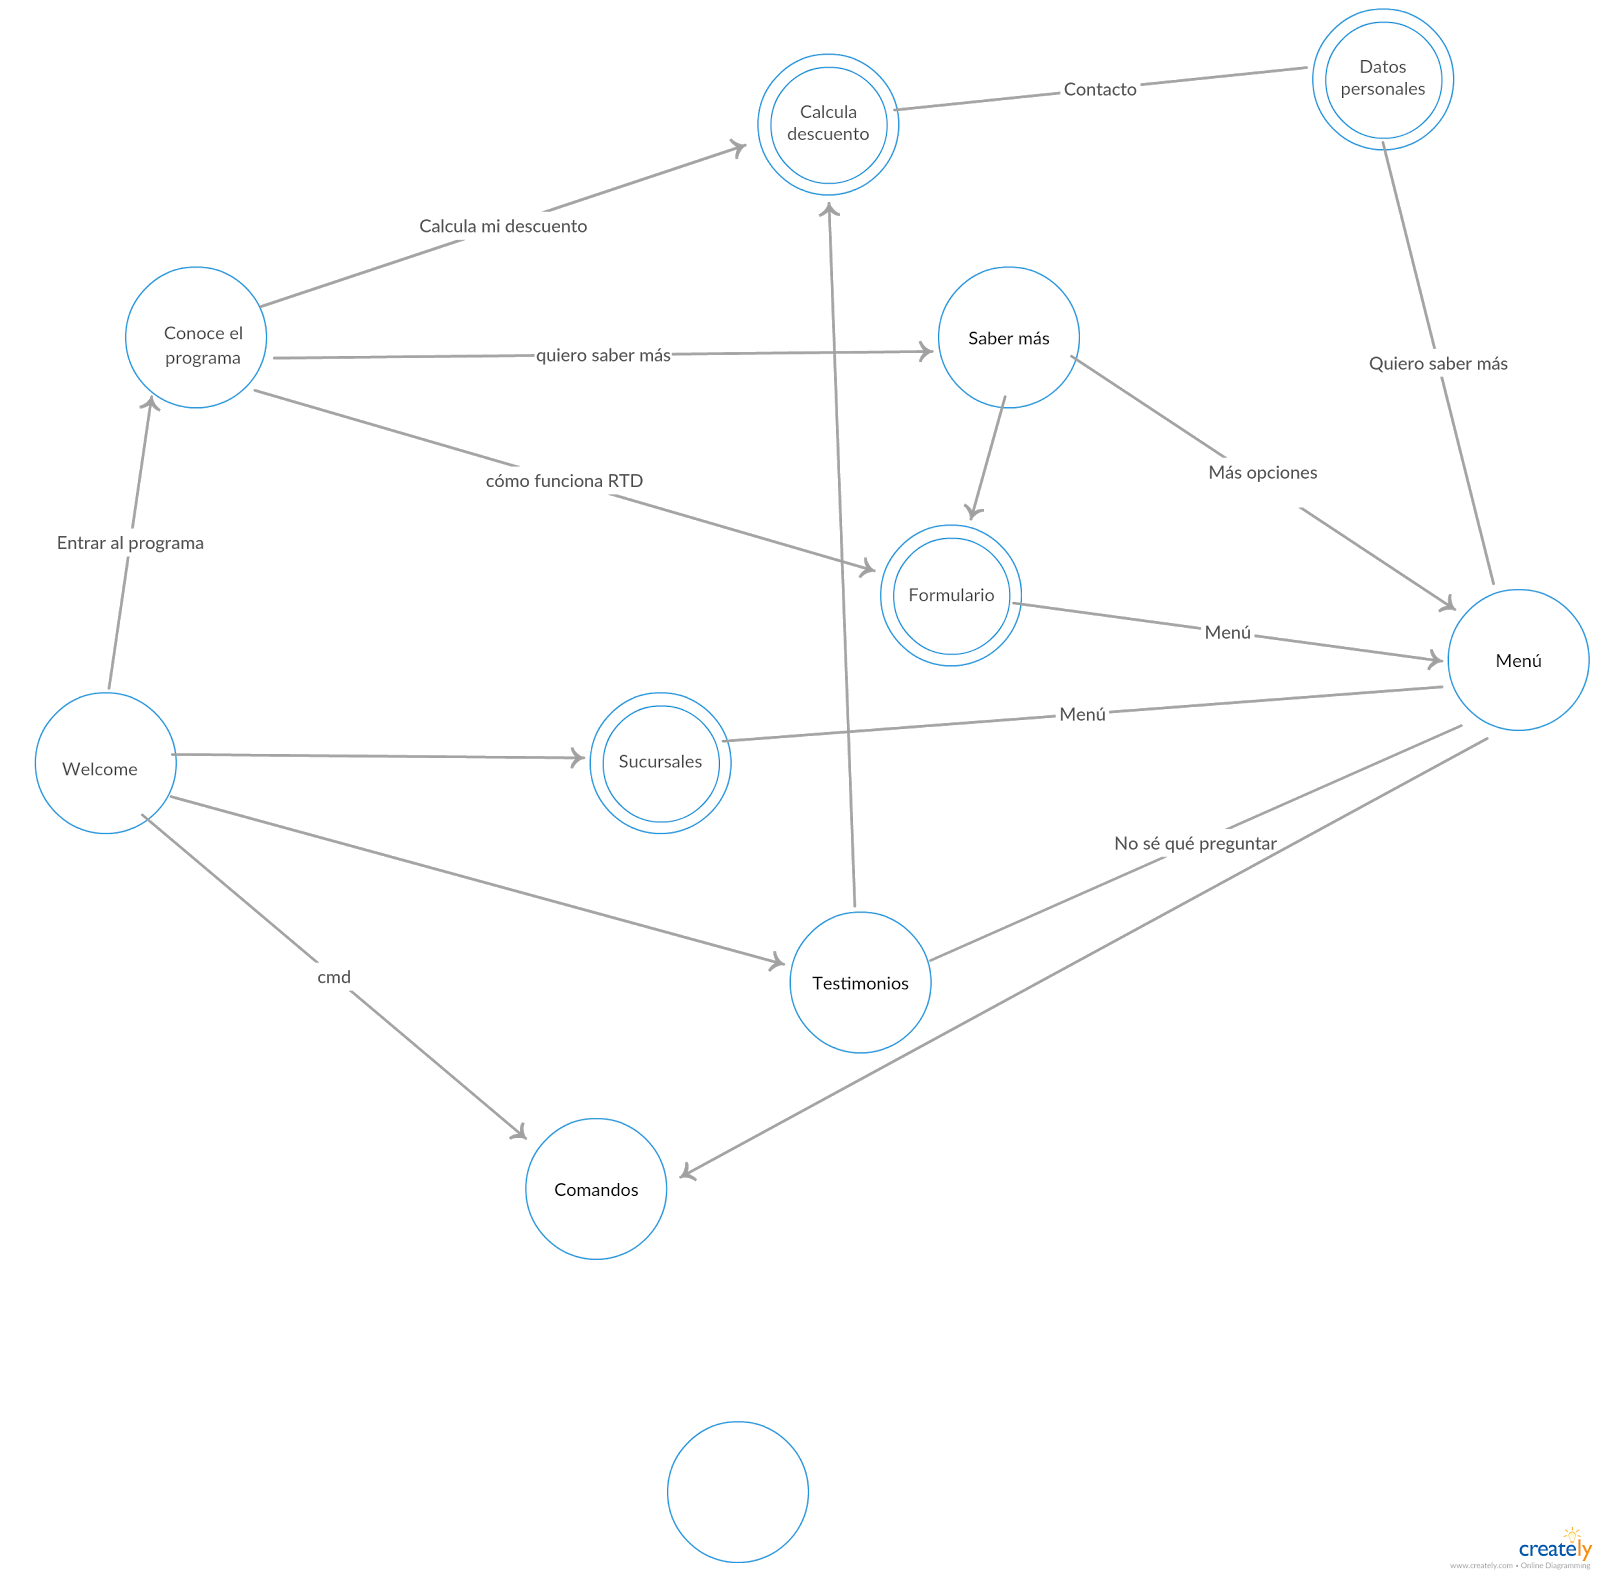
\includegraphics[width=\textwidth]{grafoInteraccion.jpg}
